\documentclass[11pt, sans, handout]{beamer}

\usepackage[utf8]{inputenc} 
\usepackage[T1]{fontenc}
\usepackage{lmodern}
\usepackage{graphicx}
\usepackage[french]{babel}
\usepackage[many]{tcolorbox}

\newtcolorbox{RDB}[2][]{%attach boxed title to top center
               = {yshift=-8pt},
  colback      = blue!5!white,
  colframe     = blue!75!black,
  fonttitle    = \bfseries,
  colbacktitle = blue!85!black,
  title        = #2,#1,
  enhanced,
}

\usetheme{Copenhagen}

\addtobeamertemplate{footline}{\insertframenumber/\inserttotalframenumber}


\begin{document}
\title{Titre}
\maketitle

\frame{
   \frametitle{Sommaire}
   \tableofcontents[currentsubsection,sectionstyle=show/shaded,subsectionstyle=show/shaded/hide]
}

\frame{
	\frametitle{Rappel théorique}
	\framesubtitle{Base de données relationnelle}
	Dans une base de données relationelle, les données sont organisées en tables. Les colonnes de ces tables sont appelées des attributs et les lignes sont appelées des tuples.\\[.5cm]
	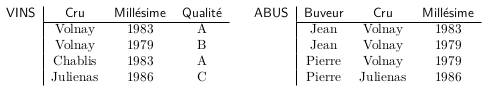
\includegraphics[scale=0.62]{RBD.png}
	Les tables d'une BDR respectent des contraintes et des clés.\\
	\begin{center}
		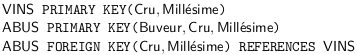
\includegraphics[scale=0.6]{BDRkeys.png}
	\end{center}
}

\frame{
	\frametitle{Rappel théorique}
	\framesubtitle{Base de données en graphe}
	Dans une base de données en graphe, les données sont contenues dans des noeuds, et les relations entre les données sont décrite par les arcs reliant ces noeuds. A chaque tupe des tables d'une BDR correspond un noeud en BDG.
}
\end{document}